\documentclass[../mathNotesPreamble]{subfiles}
\begin{document}
%  \relscale{1.4}
  \section{10.4: The Divergence and Integral Tests}

  \begin{thmBox*}[Theorem 10.9: Divergence Test]
    If $\sum a_k$ converges, then $\displaystyle\lim_{k\to \infty} a_k=0$. Equivalently, if $\displaystyle\lim_{k\to \infty} a_k\neq 0$, then the series diverges.
  \end{thmBox*}
  \begin{ex*}
    If $\displaystyle\lim_{k\to \infty} a_k=1$, what can we conclude about $\displaystyle\sum_{k=1}^\infty a_k$?
  \end{ex*}
  \vspace*{\stretch{1}}
  \begin{ex*}
    If $\displaystyle\sum_{k=1}^\infty a_k=42$, what can we conclude about $\displaystyle\lim_{k\to \infty} a_k$?
  \end{ex*}
  \vspace*{\stretch{1}}
  \begin{ex*}
    If $\displaystyle \lim_{k\to \infty} a_k=0$, what can we conclude about $\displaystyle\sum_{k=1}^\infty a_k$?
  \end{ex*}
  \vspace*{\stretch{1}}
  \pagebreak

  \begin{ex*}
    Determine which of the following series diverge by the divergence test.
  \end{ex*}
  \begin{tasks}[after-item-skip=\stretch{1}, label=,item-indent=0pt](1)
    \task $\displaystyle\sum_{k=1}^\infty \frac{1}{\sqrt{k+1}}$
    \task $\displaystyle\sum_{k=1}^\infty \frac{k^3+100}{3k^3+k+1}$
    \task $\displaystyle\sum_{k=1}^\infty \frac{e^k}{k^2}$
  \end{tasks}
  \vspace*{\stretch{1}}
  \pagebreak

  \vspace*{\stretch{1}}
  \begin{center}
    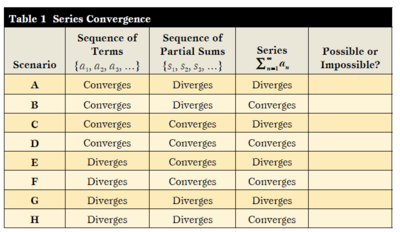
\includegraphics[width=0.8\linewidth]{../images/briggs_10_04/PossibleImpossibleSeriesTable}
  \end{center}
  \vspace*{\stretch{1}}
  \begin{thmBox*}[Theorem 10.10: Harmonic Series]
    The harmonic series $\displaystyle\sum_{k=1}^\infty\frac{1}{k}=1+\frac{1}{2}+\frac{1}{3}+\frac{1}{4}+\frac{1}{5}+\dots$ diverges---even though the terms of the series approach zero.
  \end{thmBox*}
  \pagebreak

  \begin{thmBox*}[Theorem 10.11: Integral Test]
    Suppose $f$ is a continuous, positive, decreasing function, for $x\geq 1$, and let $a_k=f(k)$, for $k=1,2,3,\dots$. Then
      \[\sum_{k=1}^\infty a_k \textnormal{ and } \int_1^\infty f(x)\,dx\]
    either both converge or both diverge. In the case of convergence, the value of the integral is \textit{not} equal to the value of the series.
  \end{thmBox*}
  \begin{ex*}
    Which of the following series below satisfy all the conditions to use the Integral Test?
  \end{ex*}
  \begin{tasks}[after-item-skip=\stretch{1}, label=,item-indent=0pt](1)
    \task $\displaystyle\sum_{k=1}^\infty \arctan(k)$
    \task $\displaystyle\sum_{k=1}^\infty \frac{(-1)^k}{k^2}$
    \task $\displaystyle\sum_{k=1}^\infty \frac{1}{e^k}$
  \end{tasks}
  \vspace*{\stretch{1}}
  \pagebreak

  \begin{ex*}
    Consider the series
      \[\sum_{k=1}^\infty \frac{1}{k^p}\]
    Use the integral test to show that the Harmonic Series diverges. For what values of $p$ does this series converge?
  \end{ex*}
  \vspace*{\stretch{1}}
  \pagebreak

  \begin{thmBox*}[Theorem 10.12: Convergence of the $p$-series]
    The \textbf{$p$-series} $\displaystyle\sum_{k=1}^\infty \frac{1}{k^p}$ converges for $p>1$ and diverges for $p\leq 1$.
  \end{thmBox*}
  \begin{ex*}
    Determine if the following $p$-series converge or diverge.
  \end{ex*}
  \begin{tasks}[after-item-skip=\stretch{1}, label=,item-indent=0pt](2)
    \task $\displaystyle \sum_{k=1}^\infty \frac{1}{k^2}$
    \task $\displaystyle \sum_{k=1}^\infty k^{-1/3}$
    \task $\displaystyle \sum_{k=1}^\infty \frac{k^2}{k^\pi}$
    \task $\displaystyle \sum_{k=1}^\infty \frac{2}{k}$
    \task $\displaystyle \sum_{k=1}^\infty \frac{-3}{\sqrt[3]{k^4}}$
    \task $\displaystyle \sum_{k=1}^\infty \frac{k^3+1}{k^5}$
  \end{tasks}
  \vspace*{\stretch{1}}
  \pagebreak

  \begin{ex*}
    Apply the Integral Test to determine if the series $\displaystyle\sum_{k=1}^\infty \frac{1}{\sqrt{k+1}}$ converges or diverges.
  \end{ex*}
  \vspace*{\stretch{1}}
  \pagebreak

  \begin{thmBox*}[Theorem 10.13: Estimating Series with Positive Terms]
    Let $f$ be a continuous, positive, decreasing function, for $x\geq 1$, and let $a_k=f(k)$, for $k=1,2,3,\dots$. Let $S=\displaystyle\sum_{k=1}^\infty a_k$ be a convergent series and let $S_n=\displaystyle\sum_{k=1}^n a_k$ be the sum of the first $n$ terms of the series. The remainder $R_n=S-S_n$ satisfies 
      \[R_n < \int_n^\infty f(x)\,dx.\]
    Furthermore, the exact value of the series is bounded as follows:
      \[L_n=S_n+\int_{n+1}^\infty f(x)\,dx < \sum_{k=1}^\infty a_k < S_n+\int_n^\infty f(x)\,dx=U_n.\]
  \end{thmBox*}
  \begin{ex*}
    How many terms of the convergent $p$-series $\displaystyle\sum_{k=1}^\infty \frac{1}{k^2}$ must be summed to obtain an approximation that is within $10^{-3}$ of the exact value of the series?
  \end{ex*}
  \vspace*{\stretch{1}}

  \pagebreak
\end{document}
